
\documentclass[12pt,a4paper]{scrartcl}

\usepackage[a4paper, left=2cm, right=1cm, bottom=1cm, top=1cm, includeheadfoot]{geometry}
\usepackage[ngerman]{babel}
\usepackage[utf8]{inputenc} % comment this if you uncomment utf8x
%\usepackage[utf8x]{inputenc} % uncomment this if there are problems with 'ä', 'ü', 'ö'
\usepackage{ucs}
\usepackage[usenames,dvipsnames]{xcolor}
\usepackage[fleqn]{amsmath}
\usepackage{amsfonts}
\usepackage{amssymb}
\usepackage{color}
\usepackage{listings}
\usepackage{hyperref}
\usepackage{amsfonts}
\usepackage{listings}
\usepackage{scrpage2}
\usepackage{graphicx}


\definecolor{mygray}{rgb}{0.9,0.9,0.9}
\lstset{language=[Visual]Basic, morekeywords={param, local}}


\lstset{
   literate={ö}{{\"o}}1
           {ä}{{\"a}}1
           {ü}{{\"u}}1
           {ß}{{\ss}}1
           {é}{{\'e}}1,
   inputencoding=ansinew,
   extendedchars=true,
   basicstyle=\scriptsize\ttfamily,
   numberstyle=\scriptsize,
   breaklines=true,
   tabsize=2,
   numbersep=5pt
}
\lstdefinestyle{customcpp}{
   language=C++,
   backgroundcolor=\color{mygray},
   numbers=left,
   keywordstyle=\color{blue}\bfseries,
   stringstyle=\color{BrickRed}\ttfamily,
   commentstyle=\color{OliveGreen}\ttfamily,
   showspaces=false,
   showstringspaces=false,
   showtabs=false
}
\lstdefinestyle{customoutput}{
   backgroundcolor=\color{mygray},
   numbers=none,
   showspaces=false,
   showtabs=false
}

\newcommand{\sourceCode}[1]{\lstinputlisting[style=customcpp]{#1}} %beinhaltet alle benötigten Packages etc.
\begin{document}
\graphicspath{{./}}

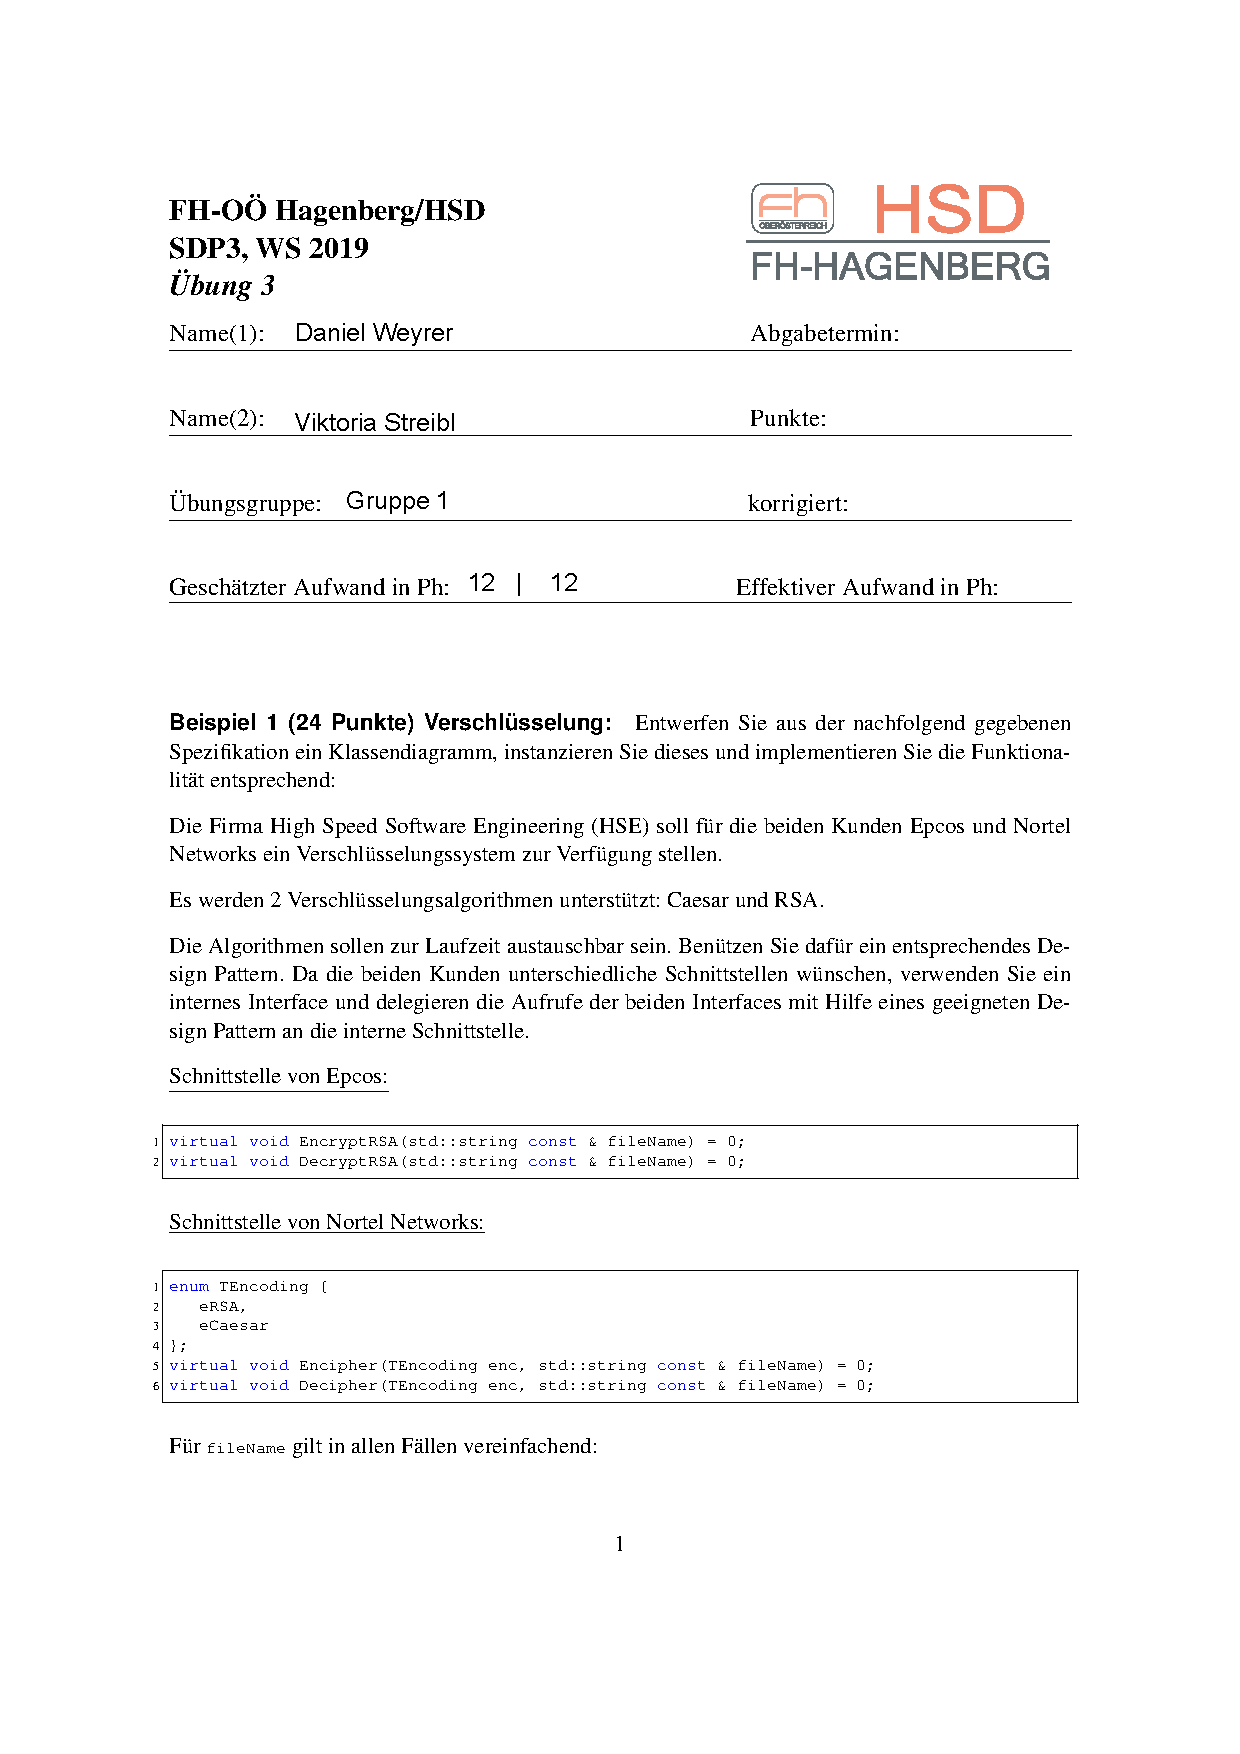
\includepdf[pages=-]{Angabe.pdf}

\title{SDP - Exercise 02} % Übungsname und Nummer angeben
\subtitle{winter semester 2019/20} % Semester angeben oder auskommentieren, falls nicht erwünscht
\author{
Viktoria Streibl - S1810306013\\
  Daniel Weyrer - S1820306044
} % Autorenname
\date{\today} % Das heutige Datum automatisch einfügen

\maketitle % Titelseite erstellen

\newpage
\tableofcontents % Inhaltsverzeichnis erstellen
\newpage

\ihead{Viktoria Streibl}
\ohead{Daniel Weyrer}
\chead{SDP3-UE Uebung 02}

\section{Organizational}
\subsection{Team}
\begin{itemize}
	\item Viktoria 	Streibl 		- 	S1810306013
	\item Daniel 	Weyrer		-	S1820306044
\end{itemize}

\subsection{Roles and responsibilities}
\subsubsection{Jointly}
\begin{itemize}
	\item Planning
	\item Documentation
	\item Systemdocumentation
	\item Class Diagram
\end{itemize}

\subsubsection{Viktoria Streibl}
\begin{itemize}
	\item Clients
	\subitem Client Nortel Networks
	\subitem Client Epos

	\item Interfaces
	\subitem IEpos
	\subitem INortelNetworks

	\item Adaptors
	\subitem AEpos
	\subitem ANorteNetworks
		
	\item Testdriver
	
\end{itemize}

\subsubsection{Daniel Weyrer}
\begin{itemize}
	\item Base Class Encryptor
	\item Derived Classes
		\subitem Class RSA
		\subitem Class Caesar
\end{itemize}

\subsection{Effort}

\subsubsection {Viktoria Streibl}
\begin{itemize}
	\item estimated: 12 ph 
	\item actually: 6 ph
\end{itemize}

\subsubsection {Daniel Weyrer}
\begin{itemize}
	\item estimated: 12 ph 
	\item actually: 8 ph
\end{itemize}

\section{Requirenment Definition(System Specification)}
The two Companies Epos and Nortel Networks should get access to a new encryption tool via two independent interfaces (which are already given in the information sheet). As the algorithms should be changeable while running the program, we came up with the idea of two adaptors and one base class.

\section{System Design}
\subsection{Classdiagram}
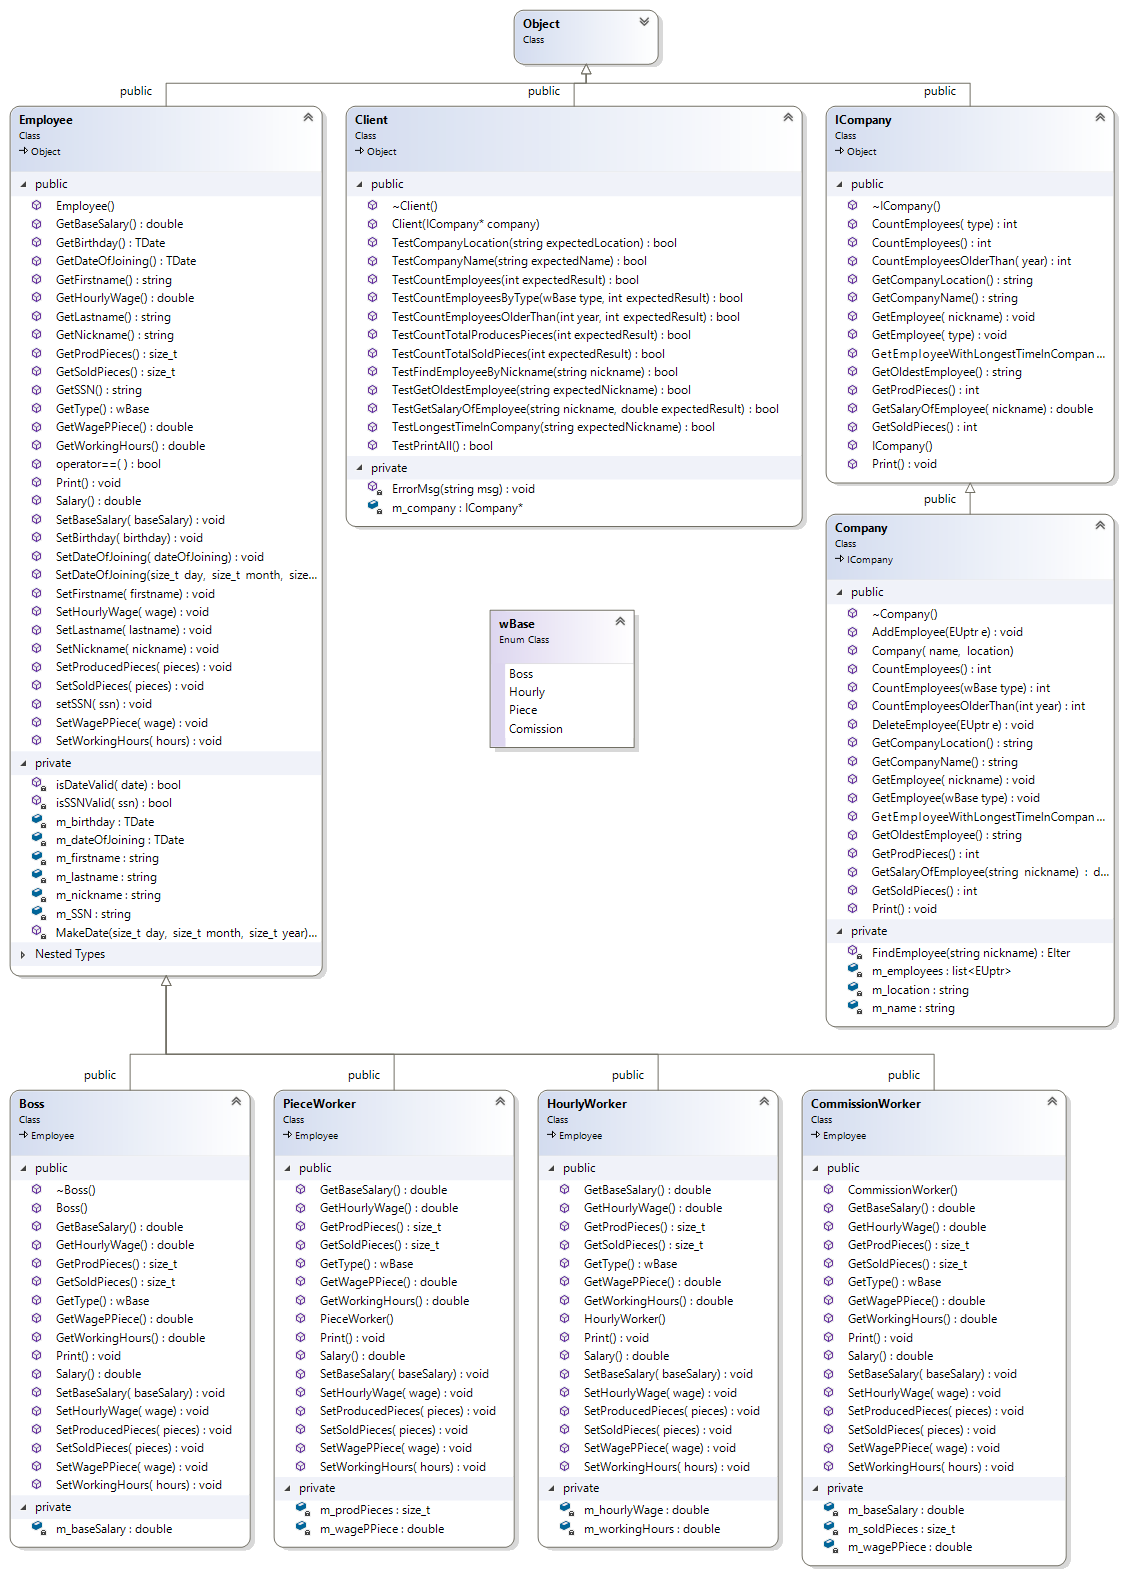
\includegraphics[scale=0.56, angle=90]{ClassDiagram}

\subsection{Design Decisions}
\subsubsection{Reading File into String}
The encryption is limited to 7-Bit ASCII-Values, which limits the encryption to plain text files. txt-files in the Megabyte-range are rare and the encryption method is not designed to deal with such many characters (+ it`s not safe, as we use a small key (RSA) and encrypt character by character).
\subsubsection{ASCII-Characters over 127}
\begin{itemize}
	\item Caesar-Encryption:	Characters with an ASCII-value over 127 cannot be encrypted due to the modulo division by 127, the Caesar-algorithm uses.	
	
	\subitem Encrypting: Characters are written unencrypted into the .Caesar with a warning written 
	\subitem in the command-line. 
	\subitem Decrypting: ASCII-values over 127 in a decrypted file (.caesar) are getting copied over to the decrypted.txt without any decryption. 
			A warning is being delivered to the command-line

	\item RSA-Encryption
	\subitem Encrypting: Characters are being ignored and a warning is being delivered to the cmd, because we found no solution 
		to handle values over 127 when decrypting a message. 
	\subitem Decrypting: All values are getting decrypted. If a decrypted-value is over 127 a warning is being delivered to 
		the command-line and the decrypted-value is stored in the decrypted.txt

\end{itemize}

\subsubsection{Exception-Handling}
\begin{itemize}
	\item badalloc (thrown by e.g. string::reserve())
	\item std::exception (thrown by systemfunctions and user)
	\item unhandled exceptions
\end{itemize}
All Exceptions are thrown in the base-class (protected, non-public functions) and captured in the derived classes!

\subsubsection{Clients}
 To make the testing easier and avoid code duplication, we decided to not test in the Client-Files this time. We created all tests in the Testdriver and used the client object for testing.
	
\section{Component Design}
\subsection{Client Epos}
This class is the for the company Epos and uses the interface IEpos.
\begin{itemize}
\item void EncryptRSA(fileName)
\subitem It calls the method EncryptRSA of the interface.
\item void DecryptRSA(fileName)
\subitem It calls the method DecryptRSA of the interface.
\end{itemize}

\subsection{Client Nortel Networks}
This class is the for the company Epos and uses the interface INortelNetworks, it contains following functions:
\begin{itemize}
\item void Encipher(type, fileName)
\subitem It calls the method Encipher of the interface.
\item void Decipher(type, fileName)
\subitem It calls the method Decipher of the interface.
\end{itemize}

\subsection{Interface IEpos}
This interface holds the following functions:
\begin{itemize}
\item virtual  void EncryptRSA(fileName)
\subitem Defines a function for encrypting a file via RSA.
\item virtual void DecryptRSA(fileName)
\subitem Defines a function for decrypting a file via RSA.
\end{itemize}

\subsection{Interface INortelNetworks}
This interface holds the following functions:
\begin{itemize}
\item virtual  void Encipher(type, fileName)
\subitem Defines a function for encrypting a file with the algorithm of the specific type.
\item virtual void Decipher(type, fileName)
\subitem Defines a function for decrypting a file with the algorithm of the specific type.
\end{itemize}

\subsection{Adaptor AEpos}
This class is an adapter for the Interface IEpos. It contains following methods:
\begin{itemize}
\item void EncryptRSA(fileName)
\subitem Implements the function of the Interface. It calls the RSA encrypting algorithmn and encrypts the file.
\item void DecryptRSA(fileName)
\subitem Implements the function of the Interface. It calls the RSA decrypting algorithmn and decrypts the file.
\end{itemize}

\subsection{ANortelNetworks}
This class is an adapter for the Interface INortelNetworks. It contains following methods:
\begin{itemize}
\item void Encipher(type, fileName)
\subitem Implements the function of the Interface. It checks which kind of encoding type it should use and calls
the respective algorithmn of encrypting.
\item void Decipher(type, fileName)
\subitem Implements the function of the Interface. It checks which kind of encoding type it should use and calls
the respective algorithmn of decrypting.
\end{itemize}

\subsection{Class Encryptor}
Base Class, contains base-functionality such as:
\begin{itemize}
\item void GenFile(fileName, content)
\subitem Creates new File with the given Filename and writes the content into the file

\item string ReadFile(fileName)
\subitem Reads of the file with the given File-name into a string and returns the string.

\item string NewFileEnding(oldFileName, oldFileEnding, newFileEnding (, appendix)
\subitem Checks for correct file-ending of the file and creates a new one with the new file-extension and optional with an appendix (to create "filename decrypted.txt"). Throws an exception if the file has the wrong file-extension, returns string with new Filename (and extension) otherwise.
\end{itemize}

\subsection{Class Caesar}
Derived class, responsible for the Caesar-Encryption
\begin{itemize}
	\item Caesar()
	\subitem Sets default encryption-key
	
	\item Encrypt(fileName)
	\subitem Main Encryptionfunction, responsible for the whole encryption process:
	\subsubitem Check file for correct ending
	\subsubitem Read file to a String
	\subsubitem create a encrypted string (character by character)
	\subsubitem create a file with the new file extension ".caesar" 
	\subsubitem Write encrypted string to the newly created file
	
	\item Decrypt(fileName)
	\subitem Main Decryptionfunction, responsible for the whole decryption process:
	\subsubitem Check for correct file extension
	\subsubitem Read File to a string
	\subsubitem create a decrypted string
	\subsubitem create a new file with "-decrypted.txt" ending and extension
	\subsubitem write the decrypted string to the newly created file
\end{itemize}
\subsection{Class RSA}
Derived class, responsible for the RSA-Encryption
\begin{itemize}
	\item Caesar()
	\subitem Sets default encryption-keys
	
	\item Encrypt(fileName)
	\subitem Main Encryptionfunction, responsible for the whole encryption process:
	\subsubitem Check file for correct ending
	\subsubitem Read file to a String
	\subsubitem create a encrypted string (character by character)
	\subsubitem create a file with the new file extension ".RSA" 
	\subsubitem Write encrypted string to the newly created file
	
	\item Decrypt(fileName)
	\subitem Main Decryptionfunction, responsible for the whole decryption process:
	\subsubitem Check for correct file extension
	\subsubitem Read File to a string
	\subsubitem create a decrypted string
	\subsubitem create a new file with "-decrypted.txt" ending and extension
	\subsubitem write the decrypted string to the newly created file
	
	\item CalcPowMod(c, pow, mod)
	\subitem Based on the RSA Algorithm, it is needed to calculate \(c^{pow} \bmod mod\). This function splits the calculation into pieces to avoid high numbers.
\end{itemize}

\subsection{TestDriver}
The Testdriver test alle functions of the clients. It tests the interface for the Epos-Company as well as the NortelNetwork-Company. It encrypt and decrypt several files. It contains also some functions:
\begin{itemize}
\item int main()
\subitem It calls all tests.

\item void CreateFullTest(subtitle, filename)
\subitem This function calls the function to print the title of the tests. Then i tests the Epos functionality and the Nortel Network functionality.

\item void testEPOS(fileName)
\subitem It calls at first the encrypting method of the specific file and than the decrypting method.

\item void testNN(type, fileName)
\subitem It calls at first the encrypting method of the specific file tests all encoding types, than it decrypts the outcome.

\item void PrintSubheader(subtitle)
\subitem This function outputs the title of the following test.
\end{itemize}
Following tests are implemented:
\begin{itemize}
\item Test alphabet and numbers
\item Test special characters
\item Testing an email file
\item Test if no file is there
\item Test if file is empty
\end{itemize}
It ouputs a error message if there was no successful run.

\newpage
\section{Test Protocol}

\subsection{Testfiles}
\subsubsection{alphabet.txt}
\sourceCode{./Encoding/testFiles/alphabet.txt}
\subsubsection{specialCharacters.txt}
\sourceCode{./Encoding/testFiles/specialCharacters.txt}
\subsubsection{email.txt}
\sourceCode{./Encoding/testFiles/email.txt}

%\subsection{Encrypted Files}
%\subsubsection{alphabet.RSA}
%\sourceCode{./Encoding/testFiles/alphabet-r.RSA}
%\subsubsection{alphabet.Caesar}
%\sourceCode{./Encoding/testFiles/alphabet-c.Caesar}
%\subsubsection{specialCharacters.RSA}
%\sourceCode{./Encoding/testFiles/specialCharacters-r.RSA}
%\subsubsection{specialCharacters.Caesar}
%\sourceCode{./Encoding/testFiles/specialCharacters-c.Caesar}
%\subsubsection{email.RSA}
%\sourceCode{./Encoding/testFiles/email-r.RSA}
%\subsubsection{email.Caesar}
%\sourceCode{./Encoding/testFiles/email-c.Caesar}

\subsection{Decrypted Files}
\subsubsection{alphabet-decrypted.txt}
\sourceCode{./Encoding/testFiles/alphabet-decrypted.txt}
\subsubsection{specialCharacters-decrypted.txt}
\sourceCode{./Encoding/testFiles/specialCharacters-decrypted.txt}
\subsubsection{email-decrypted.txt}
\sourceCode{./Encoding/testFiles/email-decrypted.txt}
\newpage
\subsection{Console Output}
\sourceCode{./Encoding/output.txt}

\newpage
\section{Source Code}

\subsection{ClientEpos}
\subsubsection{ClientEpos.h}
\sourceCode{./Encoding/Encoding/Client_Epos.h}
\subsubsection{ClientEpos.cpp}
\sourceCode{./Encoding/Encoding/Client_Epos.cpp}
\newpage
\subsection{Client Nortel Networks}
\subsubsection{ClientNortelNetworks.h}
\sourceCode{./Encoding/Encoding/Client_NortelNetworks.h}
\subsubsection{ClientNortelNetworks.h}
\sourceCode{./Encoding/Encoding/Client_NortelNetworks.cpp}
\newpage

\subsection{Interface IEpos}
\subsubsection{IEpos.h}
\sourceCode{./Encoding/Encoding/IEpos.h}

\subsection{Interface INortelNetworks}
\subsubsection{INortelNetworks.h}
\sourceCode{./Encoding/Encoding/INortelNetworks.h}
\newpage

\subsection{Adaptor AEpos}
\subsubsection{AEpos.h}
\sourceCode{./Encoding/Encoding/AEpos.h}
\subsubsection{AEpos.cpp}
\sourceCode{./Encoding/Encoding/AEpos.cpp}
\newpage
\subsection{ANortelNetworks}
\subsubsection{ANortelNetworks.h}
\sourceCode{./Encoding/Encoding/ANortelNetworks.h}
\subsubsection{ANortelNetworks.cpp}
\sourceCode{./Encoding/Encoding/ANortelNetworks.cpp}
\newpage

\subsection{Class Encryptor}
\subsubsection{Encryptor.h}
\sourceCode{./Encoding/Encoding/Encryptor.h}
\subsubsection{Encryptor.cpp}
\sourceCode{./Encoding/Encoding/Encryptor.cpp}
\newpage

\subsection{Class Caesar}
\subsubsection{Caesar.h}
\sourceCode{./Encoding/Encoding/Caesar.h}
\subsubsection{Caesar.cpp}
\sourceCode{./Encoding/Encoding/Caesar.cpp}
\newpage
\subsection{Class RSA}
\subsubsection{RSA.h}
\sourceCode{./Encoding/Encoding/RSA.h}
\subsubsection{RSA.cpp}
\sourceCode{./Encoding/Encoding/RSA.cpp}
\newpage

\subsection{TestDriver}
\subsubsection{TestDriver.h}
\sourceCode{./Encoding/Encoding/TestDriver.h}
\subsubsection{TestDriver.cpp}
\sourceCode{./Encoding/Encoding/TestDriver.cpp}
\newpage
% Um Quellcode einzufügen einfach diesen Befehl verwenden:
%\sourceCode{Relativer/Pfad/zum/SourceCode.Endung}

\end{document}